% !TEX encoding = UTF-8 Unicode
% !TEX TS-program = LuaLaTeX
% !TEX root = ../memoire.tex
% !TEX spellcheck = fr-FR

%************************************************
\chapter{Apprentissage statistique}
\label{chap:deux}
%************************************************

\section{Théorie}

\subsection{L'apprentissage machine}

Initialement une branche des statistiques, l'apprentissage statistique s'est rapidement transformé en une discipline à part entière mêlant plusieurs domaines des mathématiques et de l'informatique: l'apprentissage machine.

Le terme \emph{apprentissage statistique} en lui-même est vague et regroupe plusieurs sous-domaines. De façon générale on dispose d'un échantillon $\mathcal{L}$ d'individus possédant des caractéristiques $X_i \in \mathcal{X}$ propres considérées comme déterministes appelées variables et un attribut aléatoire $Y \in \mathcal{Y}$. Si $\mathcal{Y}$ est un ensemble discret on parle de problème de \emph{classification}, s’il est continu on parle alors de problème de \emph{régression}. Il existe un grand nombre d'autres objectifs comme le \emph{clustering}, la \emph{détection de structures} et autres, mais nous ne nous intéresserons ici qu'à ces deux grandes familles en choisissant à chaque fois la tache qui facilite les explications ou est la plus en rapport avec notre problème.

Il est possible de distinguer deux grandes approches pour l'apprentissage machine:
\begin{description}
    \item[L'estimation statistique] est l'approche classique et historiquement la première approche. Ici le but est d'\emph{identifier} la fonction génératrice\sidenote{Ici on appelle \emph{fonction génératrice} la densité ou probabilité qui donne naissance aux individus, et non la fonction (ou \textquote{\emph{système}}) qui lie les caractéristiques d'un individu à son attribut.} des données parmi une classe de fonction choisies. Un certain nombre d'hypothèses doit être fait puis à l'aide de techniques d'approximation fonctionnelle le modèle le plus probable est choisi parmi ceux considérés. Il est possible de différencier l'estimation paramétrique ou une classe de fonctions génératrices est fixée et le problème se ramène à l'estimation des paramètres de ces fonctions, et l'estimation non paramétrique ou aucune hypothèse sur la fonction génératrice des données n'est faite. L'estimation non paramétrique paraît a priori plus attirante puisque souvent il est impossible de connaître la famille à laquelle appartient la fonction génératrice, néanmoins les résultats ne sont valides qu'asymptotiquement et un nombre d'observations bien plus important que dans le cas de l'estimation paramétrique est nécessaire.
    \item[L'apprentissage prédictif,] qui s'occupe d'\emph{imiter} le \emph{système} qui pour chaque individu est capable d'associer l'attribut aux caractéristiques. Le but est ici la création d'un modèle non pas \textquote{vrai} mais qui se \emph{généralise}, c'est-à-dire à même d'obtenir les mêmes performances sur de nouveaux individus non observés que sur l'échantillon $\mathcal{L}$.
\end{description}

Le problème d'apprentissage prédictif est plus simple que le problème classique d'estimation statistique puisque l'on ne cherche pas à trouver le vrai modèle, mais seulement une assez bonne imitation. Les deux approches ne cherchent pas à répondre à la même question et ne peuvent donc pas être comparées directement. Résoudre le problème d'estimation statistique permet de comprendre toutes les caractéristiques du système et les étudier, ce que le problème d'apprentissage statistique n'a pas vocation à faire puisqu'il ne cherche qu'à répliquer le pouvoir prédictif du système. Dans le cas de la classification ou de la régression nous ne sommes intéressés que par la capacité de notre \emph{classifieur} ou \emph{régresseur} à obtenir de bonnes performances sur de nouveaux individus, le concept de \emph{bonnes performances} étant à définir en fonction du problème. Il s'agit donc de l'approche que nous adopterons.

\begin{remark}{Plus d'informations}
    Pour plus de littérature sur l'apprentissage statistique il est possible de se référer à \citet{Trevor} ou \citet{Bishop2006} pour un aperçu des différentes méthodes d'apprentissage machine. Un traitement purement statistique de méthodes d'apprentissage ainsi qu'un traitement des techniques nécessaires à leur compréhension est disponible dans \citet{Wasserman2004}, \citet{Devroye1997} traitent de manière rigoureuses les différentes considérations mathématiques de l'apprentissage statistique. Si au contraire le lecteur cherche un aperçu plus général combinant à la fois estimation statistique et apprentissage prédictif en expliquant les motivations sans trop de lourdeur mathématique il est possible de se référer à \citet{Cherkassky2007}.
    Enfin un traitement rigoureux du cas de l'estimation paramétrique et des problèmes de convergences de telles méthodes est disponible dans \citet{Tsybakov2009}.
\end{remark}

\subsection{Minimisation du risque empirique}

Supposons que l'on possède un échantillon d'apprentissage $\mathcal{L}$ composé de $N$ individus $(\mathbf{x},y) \in \mathcal{X} \times \mathcal{Y}$. Il est possible d'essayer de modéliser la loi jointe de $(\mathbf{x},y)$ mais c'est un problème trop complexe et en réalité pas nécessaire à notre but, il suffit en effet de modéliser le lien entre $\mathbf{x}$ et $y$, c'est-à-dire considérer le problème comme l'apprentissage d'une fonction $f$ inconnue telle que $y = f (\mathbf{x}) + \varepsilon$ où $\varepsilon$ est une \emph{erreur}. Il s'agit d'une forme plus contraignante, mais en réalité plus adaptée à notre problème et beaucoup plus simple à étudier. Puisqu'il est souvent impossible de connaître la forme de la loi de $X$ ou $\varepsilon$, nous allons effectuer comme unique hypothèse que les variables sont indépendantes et de même loi.

Le problème est alors maintenant un problème d'approximation de $f$ par une famille de fonctions et un algorithme de notre choix. Nous appellerons $\varphi_{\mathcal{L}}$ l'approximation que nous obtenons de cette façon, celle-ci dépend évidemment non seulement de $\mathcal{L}$ mais de l'algorithme d'apprentissage utilisé. Puisqu'il s'agit d'un problème d'approximation fonctionnelle le cadre naturel est de se donner une distance à minimiser, mais puisque nous ne connaissons pas $f$ mais seulement les réalisations de $f$ à certains points il nous faut remplacer la distance entre les fonctions par une forme plus faible: la \emph{perte} $L$ aux points de la fonction. Ainsi la perte au point $(\mathbf{x}_i,y_i)$ est:
\begin{equation*}
    L(\varphi_{\mathcal{L}} (y_i,\mathbf{x}_i))
\end{equation*}
Enfin puisque nous disposons d'un échantillon d'apprentissage et non pas seulement d'un individu unique il semble naturel de chercher à minimiser la perte moyenne
\begin{equation*}
    \mathrm{Err} \left( \varphi  \right) = \mathbb{E}_{X,Y} \left[ L(\varphi_{\mathcal{L}} (Y,X)) \right]
\end{equation*}
Ainsi si un certain algorithme d'apprentissage est capable de modéliser une classe $\Phi$ de fonctions, notre problème est le choix d'un $\varphi_{\mathcal{L}}^\star$ tel que:
\begin{align*}
    \varphi^\star &= \argmin_{\varphi_{\mathcal{L}} \in \Phi} \mathbb{E}_{X,Y} \left[ L\left(Y,\varphi_{\mathcal{L}}\left(X\right)\right) \right] \\
    &\simeq \argmin_{\varphi_{\mathcal{L}} \in \Phi} \frac{1}{N} \sum_{i=1}^N L\left(y_i,\varphi_{\mathcal{L}}\left(\mathbf{x}_i\right)\right)
\end{align*}
Notons alors
\begin{align*}
    &\mathrm{Err}_N \left( \varphi_{\mathcal{L}} \right) = \frac{1}{N} \sum_{i=1}^N L\left(y_i,\varphi_{\mathcal{L}}\left(\mathbf{x}_i\right)\right) \\
    &\varphi_{\mathcal{L}}^\star = \argmin_{\varphi \in \Phi} \mathrm{Err}_N \left( \varphi  \right)
\end{align*}

La question naturelle est alors de se demander si les performances, c'est-à-dire la perte minimale obtenue par notre algorithme d'optimisation sur l'échantillon d'apprentissage, se généralisent sur la population totale. Il est en réalité possible de fournir des garanties pour qu'optimiser en moyenne empirique sur l'échantillon, c'est-à-dire travailler par \ac{erm}, revienne à une erreur prés à optimiser en moyenne. On veut alors prouver que notre fonction se \emph{généralise} bien, c'est-à-dire soit assez expressive pour imiter la fonction $f$ mais néanmoins assez restreinte pour ne pas donner un $\varphi$ qui colle parfaitement à l'échantillon d'apprentissage au détriment d'un pouvoir de généralisation nul.

En effet il est facile de voir que si $\Phi$ est l'ensemble de toutes les fonctions alors la perte empirique minimale sera toujours $0$ sans aucune garantie sur la perte réelle. Au contraire si l'on prend à l'inverse le cas très restreint de $\Phi = \{\text{fonctions constantes}\}$ alors les deux pertes seront relativement proches. Il faut alors introduire une notion de classes de complexité des fonctions.

C'est dans cette optique que V. Vapnik et A. Chervonenkis ont introduit la notion de \ac{vc} \citep{Vapnik1998,Vapnik2000}.
Commençons par définir la notion de \emph{consistance}:

\begin{definition}
    La procédure \ac{erm} est consistante si:
    \begin{align*}
        \mathrm{Err} \left( \varphi_{\mathcal{L}}^\star \right) \xrightarrow[\vert \mathcal{L} \vert \to +\infty]{\mathbb{P}} \mathrm{Err} ( \varphi^\star ) \\
        \mathrm{Err}_N \left( \varphi_{\mathcal{L}}^\star \right) \xrightarrow[\vert \mathcal{L} \vert \to +\infty]{\mathbb{P}} \mathrm{Err} ( \varphi^\star )
    \end{align*}
\end{definition}

Vapnik et Chervonenkis ont alors montré le théorème suivant:

\begin{theoreme}[Théorème fondamental de l'apprentissage]
    Pour une fonction de perte $L$ bornée, la méthode \ac{erm} est consistante si et seulement si le risque empirique converge uniformément vers le vrai risque, c'est-à-dire:
    \begin{equation}
        \lim_{\vert \mathcal{L} \vert \to +\infty} \mathbb{P} \left( \sup_{\varphi \in \Phi} \vert \mathrm{Err} ( \varphi_{\mathcal{L}} ) - \mathrm{Err}_N ( \varphi_{\mathcal{L}} ) \vert > \varepsilon \right) = 0 \label{equ:vc.consistant}
    \end{equation}
\end{theoreme}

On peut remarquer que~\ref{equ:vc.consistant} dépend de la classe de fonction choisie et donc que le supremum de l'erreur dépend de la richesse de la classe de fonction.

Notons alors $N(\Phi,\mathcal{L})$ le nombre de dichotomies que peuvent engendrer les fonctions de $\Phi$, aussi appelé \emph{diversité}. On peut alors définir l'\emph{entropie aléatoire}:
\begin{equation*}
    H( \Phi,\mathcal{L} ) = \ln N( \Phi,\mathcal{L} )
\end{equation*}
et l'entropie de Vapnik-Chervonenkis
\begin{equation*}
    H(\Phi,N) = \mathbb{E} \left[ \ln N( \Phi,\mathcal{L} ) \right]
\end{equation*}
Cette quantité dépend de la distribution de $\mathcal{L}$, on introduit alors la \emph{fonction de croissance} $G$:
\begin{equation*}
    G(\Phi,N) = \ln \max_{\mathcal{L}} N(\Phi,\mathcal{L} ) 
\end{equation*}
ainsi que l'entropie de Vapnik-Chervonenkis recuite:
\begin{equation*}
    H_{\text{recuite}} (\Phi,N) = \ln \mathbb{E} \left[ N(\Phi,\mathcal{L} ) \right]
\end{equation*}

Vapnik et Chervonenkis ont alors montré le résultat suivant:

\begin{prop}
    La procédure \ac{erm} est consistante si et seulement si
    \begin{equation*}
        \lim_{N \to +\infty} \frac{H(\Phi,N)}{N} = 0
    \end{equation*}    
\end{prop}

Cette propriété n'est en général d'aucune utilité puisqu'elle dépend de la distribution de $\mathcal{L}$ et ne donne aucune garantie sur la vitesse de convergence. On va alors chercher à trouver des conditions pour la convergence rapide:

\begin{definition}
    On dit qu'il y a \emph{convergence rapide} si il existe un $c > 0$ tel que $\forall n > n_0$:
    \begin{equation*}
        \mathbb{P} \left( \sup_{\varphi \in \Phi} \vert \mathrm{Err} ( \varphi_{\mathcal{L}} ) - \mathrm{Err}_N ( \varphi_{\mathcal{L}} ) \vert > \varepsilon \right) \leq e^{-c n \varepsilon^2}
    \end{equation*}
\end{definition}
On a alors que
\begin{equation*}
    \lim_{N \to +\infty} \frac{H_{\text{recuite}}(\Phi,N)}{N} = 0
\end{equation*}
est une condition suffisante pour la convergence rapide. Finalement:
\begin{theoreme}
    La procédure \ac{erm} est consistante et converge rapidement si et seulement si
    \begin{equation*}
        \lim_{N \to +\infty} \frac{G(\Phi,N)}{N} = 0
    \end{equation*}
\end{theoreme}

\subsection{Dimension de Vapnik-Chervonenkis}

Il est en fait possible d'obtenir des bornes de convergence explicite, pour cela il faut définir la \ac{vc}.

\begin{definition}[Dimension de Vapnik-Chervonenkis]
    On dit qu'une famille de fonctions indicatrices \emph{pulvérise} $\mathcal{L}$ si toutes les dichotomies de $\mathcal{L}$ sont réalisables par cette famille. C'est à dire dans le cas de la classification binaire que toutes les partitions en $2$ sous-ensembles de points sont possibles.
    On dit qu'une famille d'indicatrices est de \ac{vc} $h$ s’il existe un $\mathcal{L}, \vert \mathcal{L} \vert = h$ qui puisse être pulvérisé, mais pas de $\mathcal{L}, \vert \mathcal{L} \vert = h+1$. La \ac{vc} est donc le nombre maximal de dichotomies que la famille d'indicatrices puisse réaliser.
    Soit une famille de fonctions $f$ à valeurs réelles indexée par $\omega$. La \ac{vc} de $(f_\omega)$ est définie comme la \ac{vc} de la famille $\left(\mathds{1}_{ f_\omega (\cdot) - \beta > 0}\right)_{\omega,\beta}$ indexée par $\omega$ et $\beta$.
\end{definition}

\begin{figure}
    \centering
    \begin{tikzpicture}
    \begin{axis}[domain=0:1]
        \addplot[no markers, smooth, samples = 100] {sin(31.9*deg(x))};
        \addplot+[only marks, mark size = 0.5pt, blue] table [x = x, y = y, col sep = comma] {images/shatter.csv};
        \addplot+[only marks, mark size = 0.5pt, red] table [x = x, y = y, col sep = comma] {images/shatter2.csv};
    \end{axis}
    \end{tikzpicture}
    \caption{$\sin ( \omega x)$ possède un unique paramètre et une dimension VC infinie.}
\end{figure}

Vapnik et Chervonenkis ont montré que:
\begin{equation*}
    G(\Phi,N) \leq h \left( 1 + \ln \left( \frac{N}{h} \right) \right)
\end{equation*}

Le résultat le plus important, celui qui justifie de se ramener à un problème d'optimisation de la perte empirique en ignorant les habituelles questions statistiques.

\begin{theoreme}\label{thrm:vc}
    Dans le cas de la classification binaire et avec la perte $0/1$ on a:
    \begin{align}
        &\mathbb{P} \left( \sup_{\varphi \in \Phi} \vert \mathrm{Err}_N ( \varphi ) - \mathrm{Err} ( \varphi ) \vert > \varepsilon \right) \leq 8 G(\Phi,N) e^{-N \varepsilon^2 / 32} \\
        &\mathbb{E} \left[ \sup_{\varphi \in \Phi} \vert \mathrm{Err}_N ( \varphi ) - \mathrm{Err} ( \varphi ) \vert \right] \leq 2 \sqrt{\frac{\log G(\Phi,N) + \log 2 }{N}}
    \end{align}
\end{theoreme}

\begin{hproof}
    La preuve utilise la plupart des techniques courantes pour les preuves de la théorie de Vapnik-Chervonenkis et est donc adaptée et reproduite de \citet{Devroye1997} en annexe~\ref{preuve:vc}. Celle-ci procède en $4$ étapes types:
    \begin{enumerate}
        \item Symétrisation par échantillon fantôme.
        \item Symétrisation par processus de Rademacher.
        \item Conditionnement sur $\mathcal{L}$.
        \item Utilisation d'une inégalité de concentration.
    \end{enumerate}
\end{hproof}

\section{Sélection du modèle}

Le choix du modèle à utiliser est un problème complexe qui dépend grandement des données en question, il n'est pas possible de trouver un modèle qui assure les meilleures performances dans tous les cas, il n'y a pas de \emph{Free Lunch} possible \citep{Wolpert1996}. Il faut donc bien comprendre comment chaque algorithme obtient de bonnes performances sur un certain jeu de données et de mauvaises sur un autre, mais surtout comprendre quels sont les éléments généraux qui gouvernent la performance des algorithmes.

\subsection{Dilemme Biais-Variance}

Le choix d'une famille de modèles ou même des hyper paramètres au sein de cette famille comme le coefficient de pénalisation, le nombre de fonctions de la base ou la bande passante d'un noyau, influent sur la complexité du modèle, où la complexité réfère ici à l'étendue des fonctions que le modèle peut représenter. Il est tentant d'augmenter la complexité d'un modèle puisqu'en pouvant représenter plus de fonctions différentes on augmente les chances de bien approcher la fonction sous-jacente, mais cela n'est pas nécessairement judicieux.

Tous les algorithmes d'apprentissage statistique cherchent d'une façon ou d'une autre à minimiser une fonction de perte sur les données d'apprentissage; le choix d'un modèle complexe et donc d'une large famille d'estimateurs permet alors mécaniquement de réduire l'erreur d'apprentissage, mais ne garantit pas forcément une réduction de l'erreur de généralisation. En effet il est possible de \emph{sur apprendre} les données d'apprentissage (\emph{overfitting}) en construisant un modèle qui s'adapte aux caractéristiques uniques de l'échantillon d'apprentissage et ne se généralise pas du tout à des données nouvelles. Il faut donc trouver un compromis entre sur et sous-apprentissages (over/under-fitting) afin d'obtenir de bonnes performances de généralisation.

\todo{on peut aussi faire le lien avec Vapnik}

Les concepts de sous et sur apprentissage sont intimement liés à la décomposition biais-variance de l'erreur de généralisation. Ainsi pour la perte quadratique on a:
\begin{equation*}
    \mathrm{Err} \left(\varphi_{\mathcal{L}} (x_0) \right) = \mathrm{Var} [y_0 \mid x_0 ] + \mathrm{Var}_{\mathcal{L}} [\hat{y}_0] + \left( f (x_0) − \mathbb{E}_{\mathcal{L}} \left[ \varphi_{\mathcal{L}} (x_0) \right] \right)^2
\end{equation*}
avec $y_0 = f (x_0) + \varepsilon$ et $\varphi_{\mathcal{L}}$ le classifieur appris sur l'échantillon d'apprentissage.

Prenons par exemple comme classifieur les $k$-plus proches voisins, on a alors \citep{Trevor}:
\begin{equation*}
    \mathrm{Err} \left( \varphi_{\mathcal{L},k} (x_0) \right) = \sigma^2 + \left[ f(x_0) - \frac{1}{k} \sum_{l=1}^k f(x_{(l)}) \right]^2 + \frac{\sigma^2}{k}
\end{equation*}

Dans le cas où la taille de l'échantillon d'apprentissage tend vers $+ \infty$ et donc la distance entre $x_0$ et $x_{(1)}$ tend vers $0$ on peut voir que le terme $\left[ f(x_0) - \frac{1}{k} \sum_{l=1}^k f(x_{(l)}) \right]^2$ est minimal pour $k=1$, puis croit vers $\left[ f(x_0) - \hat{f(x)} \right]^2$ alors que $\frac{\sigma^2}{k}$ tend vers $0$ pour $k \to \infty$. On s'aperçoit ici de la nécessité de choisir une valeur raisonnable de $k$ qui minimise la somme des deux. En effet lors de l'apprentissage l'erreur mesurée est l'erreur sur le premier terme seulement et tend vers $0$ si $k$ est choisi trop petit, il faut donc minimiser une approximation de l'erreur de généralisation. Parmi de telles approximations, les plus courantes sont:
\begin{description}
    \item[Erreur \ac{loo}] Ici le classifieur est construit sur tous les individus sauf l'individu $i$ puis l'erreur $\mathrm{LOO}_i$ est mesurée sur cet individu. L'approximation de l'erreur est alors $\mathrm{LOO} = \frac{1}{N} \sum_{i=1}^N \mathrm{LOO}_i$
    \item[Erreur \ac{k-cv}] L'erreur \ac{loo} étant incroyablement coûteuse en terme de calcul il est possible d'utiliser à la place la validation croisée: l'échantillon d'apprentissage est découpé en $k$ strates $\mathcal{L}_1,\dotsc,\mathcal{L}_k$ de tailles environ égales, le classifieur est construit sur $\mathcal{L}_{-i} = \mathcal{L} \smallsetminus \mathcal{L}_i$ et l'erreur $\mathrm{CV}_i$ mesurée sur $\mathcal{L}_i$. L'erreur \ac{k-cv} est alors $\mathrm{CV} = \frac{1}{k} \sum_{i=1}^k \mathrm{CV}_i$.
    \item[Erreur \ac{k-cv} répétée] Dans ce cas, le processus de validation croisée est moyenné sur $V$ répétitions.
\end{description}

\begin{figure}[htbp]
    \makebox[\textwidth][c]{
    \begin{tikzpicture}
    \begin{axis}[%
    name=plot1,
    domain=0:2*pi, ymin=-1.2, ymax = 1.2]
    \addplot[no markers, smooth] {sin(deg(x))};
            \foreach \yindex in {2,...,21}
                \addplot[no markers, smooth, blue, thick, opacity = 0.2] table [x index = 1, y index = \yindex, col sep = comma] {images/model1.csv};
    \end{axis}

    \begin{axis}[%
    name=plot2,
    at=(plot1.right of south east), anchor=left of south west,
    domain=0:2*pi, ymin=-1.2, ymax = 1.2]
    \addplot[no markers, smooth] {sin(deg(x))};
            \foreach \yindex in {2,...,21}
                \addplot[no markers, smooth, blue, thick, opacity = 0.2] table [x index = 1, y index = \yindex, col sep = comma] {images/model3.csv};
    \end{axis}

    \begin{axis}[%
    name=plot4,
    at=(plot2.below south west), anchor=above north west,
    domain=0:2*pi, ymin=-1.2, ymax = 1.2]
    \addplot[no markers, smooth] {sin(deg(x))};
            \foreach \yindex in {2,...,21}
                \addplot[no markers, smooth, blue, thick, opacity = 0.2] table [x index = 1, y index = \yindex, col sep = comma] {images/model20.csv};
    \end{axis}

    \begin{axis}[%
    name=plot3,
    at=(plot4.left of south west), anchor=right of south east,
    domain=0:2*pi, ymin=-1.2, ymax = 1.2]
    \addplot[no markers, smooth] {sin(deg(x))};
            \foreach \yindex in {2,...,21}
                \addplot[no markers, smooth, blue, thick, opacity = 0.2] table [x index = 1, y index = \yindex, col sep = comma] {images/model5.csv};
    \end{axis}
    \end{tikzpicture}
    }
    \caption{Apprentissage de $\sin (x)$ sur $[0,2 \pi]$ à l'aide de polynômes de degrés $1$,$3$,$5$ et $20$.}\label{fig:biaisvar}
\end{figure}

\subsection{Fléau de la dimension}

Un grand nombre d'algorithmes d'apprentissage repose sur l'utilisation d'un voisinage du point à estimer. Ces techniques, bien qu'intuitives et efficaces, voient leurs performances chuter de façon dramatique avec la dimension de $\mathcal{X}$, l'espace ambiant. En effet, supposons par exemple que les individus soient uniformément distribués sur $[0,1]^p$, alors pour créer un voisinage (au sens $L^1$ par exemple) d'une observation contenant une fraction $r$ des observations totales il faut en moyenne couvrir sur chaque dimension $r^{1/p}$. On voit ainsi dans~\ref{fig:distance.haute.dim} que très rapidement lorsque $p$ augmente il devient nécessaire de prendre en compte la majorité des réalisations de chaque variable.

\begin{figure}[htbp]
    \centering
     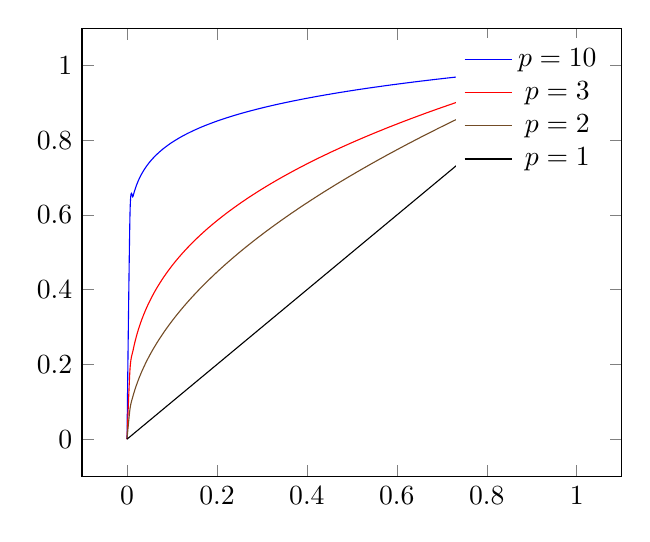
\begin{tikzpicture}
        \begin{axis}[domain=0:1, cycle list name=color, legend entries={$p=10$,$p=3$,$p=2$,$p=1$}, legend style={draw=none}, samples = 150]
            \addplot+[no markers, smooth] {x^(1/10)};
            \addplot+[no markers, smooth] {x^(1/3)};
            \addplot+[no markers, smooth] {x^(1/2)};
            \addplot+[no markers, smooth] {x};
        \end{axis}
    \end{tikzpicture}
    \caption{Évolution de la longueur moyenne des voisinages dans chaque dimension}\label{fig:distance.haute.dim}
\end{figure}


Il est, en partie également possible d'avoir l'intuition du dilemme biais-variance dans la formulation du théorème~\ref{thrm:vc} qu'une augmentation de la complexité du modèle résulte en une réduction de l'erreur empirique (biais) mais une augmentation de la borne de généralisation (assimilable à la variance). Il faut donc fixer un modèle de \ac{vc} la plus faible possible à erreur fixée, ce qui est le principe de \ac{srm}.

Qui plus est la densité de l'échantillon est proportionnelle à $N^{1/p}$. Un échantillon dense en dimension $1$ pourra alors être épars en dimension $10$.

\begin{figure}[htbp]
    \centering
    \begin{tikzpicture}
        \draw[blue,very thick] (4,0) -- (4,4);
        \draw[red,very thick] (4,0) -- (4,1);
    
        \draw[blue,thick] (5,0) rectangle (9,4);
        \draw[red,thick,fill = red!20] (5,0) rectangle (7,2);
    
        \tikzcuboidset{hidden edges/.style={dashed}}
        \pic[thick,blue] (cuboid) at (10,0,0) {cuboid=4--4--4};
        
        \tikzcuboidset{hidden edges/.style={dashed},all faces/.style={fill=red}}
        \pic[thick,red,fill opacity = 0.2] (cuboid) at (10,0,0) {cuboid=2.52--2.52--2.52};
    \end{tikzpicture}
    \caption{Un voisinage de $1/4$ de l'espace en dimensions $1$,$2$ et $3$.}
\end{figure}

Il est possible de se rendre compte de l'impact de la dimension sur différentes méthodes d'apprentissage classique \citep{Trevor}. Ainsi dans le cas des plus proches voisins, si l'on fait l'hypothèse que les observations sont distribuées uniformément sur $[0,1]^p$, la distance médiane du plus proche voisin de l'origine est de $\left( 1 - \left( \frac{1}{2} \right)^{1/N} \right)^{1/p}$. En grande dimension, les observations sont alors plus proches de la frontière que de toute autre observation.

Même un algorithme aussi simple que la régression linéaire n'est pas immunisée contre le fléau de la dimension \citep{Trevor}, supposons par exemple que les données suivent un vrai modèle linéaire c'est-à-dire que:
\begin{equation*}
    Y = X \beta + \varepsilon
\end{equation*} 
avec $\varepsilon \sim \mathcal{N}(0,\sigma^2 I)$. On a alors $\hat{y}_0 = x \hat{\beta}$ et donc $\hat{y}_0 = x_0 \beta +  x_0 ( X^\intercal X )^{-1} X^\intercal \varepsilon $ on obtient la décomposition biais-variance (voir~\ref{sec:biais.var}) on a alors
\begin{equation*}
    \mathrm{Err} (x_0) = \sigma^2 + \mathbb{E}_{\mathcal{L}} \left[ x_0^\intercal \left( X^\intercal X \right)^{-1} x_0  \right] \sigma^2 + 0^2
\end{equation*}
Donc sous l'hypothèse $\mathbb{E} [X] = 0$ on a que $X^\intercal X \sim N \operatorname{Cov} (X)$ pour $N$ grand, alors:
\begin{align*}
    \mathbb{E}_{x_0} \left[ \mathrm{Err} (x_0) \right] &\sim \mathbb{E}_{x_0} \left[ \frac{x_0^\intercal \operatorname{Cov} (X)^{-1} x_0}{N} + \sigma^2 \right] \\
    &= \mathbb{E}_{x_0} \left[ \frac{\sigma^2}{N} \sum_i \sum_j \left[ \mathrm{Cov} (x)^{-1} \right]_{ij} \left[ x_0 \right]_i \left[ x_0 \right]_j + \sigma^2 \right] \\
    &= \sigma^2 \left( \frac{\mathrm{trace} \left( \mathrm{Cov} (x)^{-1} \mathrm{Cov} (x_0) \right)}{N} +1 \right) \\
    &= \sigma^2 \left( \frac{\mathrm{trace} \left( \mathbb{I}_p \right)}{N} +1 \right) \\
    &= \sigma^2 \left( \frac{p}{N} + 1 \right)
\end{align*}
On retrouve alors ce que nous avons observé plus tôt: plus la dimension est grande plus le nombre d'observations nécessaire est important.

Nous verrons néanmoins que certains modèles résistent particulièrement bien aux hautes dimensions, notamment les forêts aléatoires dont la vitesse de convergence ne dépend que du nombre de variables informatives \citep{Biau2010a,Breiman2004a}.

\todo{Parler de la réduction de l'espace? PCA, LDA?}

%\section{$k$-plus proches voisins}

\section{Modèles linéaires et logistiques}

Bien que nous nous intéressions à la classification, il est plus simple d'étudier la régression linéaire puis de se ramener à ce cas. Bien que très simples, les méthodes linéaires possèdent de nombreuses généralisations qui étendent leur pouvoir de prédiction.

Nous cherchons alors $y = f(x)$ sous une forme bien particulière:
\begin{equation*}
    f(x) = \beta_0 + \sum_{k=1}^p x_k \beta_k
\end{equation*}

Le problème est alors une estimation des paramètres $\beta_k$ optimaux. Dans le cas de la perte $L^2$, qui est le cas le plus courant de par ses caractéristiques théoriques intéressantes et sa facilité de calcul on peut trouver directement l'estimateur. En effet, en écrivant le problème sous forme matricielle:
\begin{equation*}
    \min_\beta (y-x\beta)^\intercal(y-x\beta)
\end{equation*}
on trouve comme solution
\begin{equation*}
    \hat{\beta} = (x^\intercal x)^{-1} x^\intercal y
\end{equation*}
dont on peut donner\sidenote{Le calcul ne présente aucune difficulté mais est donné en annexe.} la variance si $y = x\beta + \varepsilon$ avec $\mathbb{V} \left[ \varepsilon \right] = \sigma^2 \mathds{I}$:
\begin{gather*}
    \mathrm{Var} ( \hat{\beta} ) = (x^\intercal x)^{-1} \sigma^2 \label{equ:var.beta} \\
    \hat{\sigma}^2 = \frac{1}{N-p-1} \sum_{i=1}^N (y_i - \hat{y}_i)^2
\end{gather*}

Le choix de l'estimateur linéaire obtenu par régression $L^2$ est dû au théorème de Gauss-Markov:
\begin{definition}
    Supposons que le modèle réel est:
    \begin{align*}
        &y = x \beta + \varepsilon \\
        &\mathbb{E} ( \varepsilon_i ) = 0 , \forall i \\
        &\mathrm{Var} ( \varepsilon ) = \sigma^2 \mathbb{I} , \sigma^2 < + \infty 
    \end{align*}
    Si $\theta$  est un estimateur linéaire de $\beta$, c'est-à-dire $\theta = H y$ et non biaisé c'est-à-dire $\mathbb{E} [\theta] = \beta$ alors nécessairement:
    \begin{equation*}
        \mathrm{Var} [\theta] \geq \mathrm{Var} [\hat{\beta}]
    \end{equation*}
    où $\hat{\beta}$ est l'estimateur des moindres carrés.
\end{definition}

Comme vu précédemment la décomposition biais-variance permet de décomposer l'erreur:
\begin{equation*}
    \mathrm{Err}_{L^2} ( \theta ) = \mathrm{Var} [\theta] + \left[ \mathbb{E} [\theta] - \beta \right]^2
\end{equation*}
donc le théorème de Gauss-Markov implique que parmi les estimateurs linéaires non biaisés, celui des moindres carrés possède la perte quadratique la plus faible. Il n'est pourtant pas toujours judicieux de ne considérer que des estimateurs non biaisés, en effet le dilemme biais-variance s'applique toujours et nous verrons qu'il existe des estimateurs biaisés qui présentent une plus faible variance et peuvent donc éventuellement obtenir une perte totale plus faible.

\subsubsection{Restriction à un sous-ensemble de variables}

Une méthode courante visant à diminuer la complexité du modèle et améliorer son pouvoir de généralisation est la restriction à un sous-ensemble bien choisi de variables sur lesquelles effectuer la régression. La sélection d'un sous-ensemble optimal de variables de taille donnée étant un problème NP-difficile il convient de mettre en place des stratégies heuristiques.

La méthode la plus couramment utilisée est la sélection de variables par étape \emph{forward} ou \emph{backward}. Dans la sélection \emph{forward}, l'algorithme commence par estimer l'origine $\beta_0$ puis, à chaque étape, ajoute la variable qui maximise la réduction de l'erreur. La procédure s'arrête une fois le nombre de variables souhaitées atteint. La sélection \emph{backward} procède de la même façon, mais en retirant la variable contribuant le moins à l'ensemble en partant de l'ensemble total des variables.

Il existe également une version plus générale de l'algorithme sélection des variables: \ac{lars} \citep{Efron2003} qui peut être utilisée non seulement pour reconstruire l'algorithme \emph{forward step-wise} mais également le chemin complet du \emph{Lasso}.

\subsubsection{Restriction par pénalisation}

Une autre approche pour contrôler la complexité du modèle est d'ajouter une pénalisation sur la norme du vecteur des coefficients, et donc une restriction sur les valeurs admissibles des coefficients.

Dans le cas général, cela revient à résoudre le problème suivant
\begin{equation*}
    \argmin_\beta \left\{ (Y - X \beta)^\intercal ( Y - X \beta ) + \lambda \Vert \beta \Vert_q  \right\}
\end{equation*}
pour une norme $q \geq 1$. Dans le cas $q=2$ on obtient la pénalisation d'arête (\emph{ridge}) ou régularisation de Tychonoff qui possède une solution explicite et est donc facile à déterminer. Dans le cas $q=1$ on obtient la régression \emph{LASSO}, il s'agit d'un problème de minimisation quadratique et peut donc être également aisément calculé. Le \emph{LASSO} présente une particularité intéressante: les coefficients seront souvent fixés à une valeur exactement égale à $0$, et cette régularisation en plus d'améliorer le pouvoir de généralisation de la régression effectue donc une forme de sélection des variables automatique. Ce phénomène peut se comprendre en examinant la pénalisation sous un point de vu Bayesien \citep{Park2008}, on peut rapidement le comprendre en réécrivant le problème comme:
\begin{equation*}
    \argmax_\beta -\left\{ (Y - X \beta)^\intercal ( Y - X \beta ) - \lambda \Vert \beta \Vert_q  \right\}
\end{equation*}
Or on rappelle que l'on a dans le cadre Bayesien:
\begin{equation*}
    \log ( \text{a posteriori} ) \thicksim \log (\text{vraisemblance}) + \log(\text{a priori})
\end{equation*}
On cherche donc le mode de l'a posteriori. Dans le cas d'une erreur Gaussienne on peut donc identifier les moindres carrés à la vraisemblance et la pénalisation à l'a priori d'une certaine loi de la famille exponentielle. Lorsque $q = 1$ on obtient un a priori de Laplace~\ref{fig:laplace}.

\begin{figure}[htbp]
    \centering
    \begin{tikzpicture}
    \begin{axis}[domain=-10:10, enlargelimits = false, legend style={draw=none}, samples = 200]
        \addplot+[no markers,blue] { 1/2*exp(-abs(x)) };
    \end{axis}
    \end{tikzpicture}
    \caption{Densité de la loi de Laplace}\label{fig:laplace}
\end{figure}

Bien que les $q \in ]1,2[$ soient intéressants, car correspondant à des a priori bayesiens différents, la résolution du problème est bien trop difficile, il est alors souvent choisi comme compromis la pénalisation \emph{Elastic-Net}:
\begin{equation*}
    \argmin_\beta \left\{ (Y - X \beta)^\intercal ( Y - X \beta ) + \lambda ( \alpha \Vert \beta \Vert_2 + (1-\alpha) \Vert \beta \Vert_1 )  \right\}
\end{equation*}

\subsubsection{Régression logistique}

Il est possible d'étendre les modèles linéaires par une transformation non linéaire de l'objectif. Ainsi le nouveau modèle est
\begin{equation*}
    y = g^{-1} ( x \beta )
\end{equation*}
où $g$ est appelée la fonction de lien. Dans le cas de la classification binaire, on considère les réalisations $y$ comme une variable de Bernouilli dont on veut estimer la probabilité de réussite. On choisit comme fonction de lien
\begin{equation*}
    g(y) = \log \left( \frac{y}{1-y} \right)
\end{equation*}
En effet cette fonction, appelée \emph{logit}, mesure les \emph{odds-ratio} de la variable de Bernouilli et fournit donc une interprétation par analyse discriminante évidente: lorsque l'\emph{odds-ratio} est supérieur à $1$ on associe un succès et un échec dans le cas inférieur à $1$.

Il n'existe pas dans ce cas de formule analytique comme dans le cas linéaire simple, l'estimation de $\beta$ est alors effectué par maximum de vraisemblance et nécessite donc des calculs de minimisation par méthode de Newton-Rhapson par exemple, qui sont bien plus coûteux.

%\subsection{Analyse discriminante linéaire}

\todo{faire analyse discriminante}

\section{Machines à vecteurs de support}

Dans le cas de la discrimination, on a jusqu'à présent cherché à chaque fois à se ramener à un problème de séparation des données par un hyperplan d'une façon ou d'une autre. Il paraît donc légitime d'essayer de poser le problème sous la forme de la recherche d'un hyperplan de séparation \emph{optimal} en un certain sens à définir.

\subsection{Séparation par un hyperplan optimal}
\subsubsection{Cas séparable}

On cherche à minimiser l'erreur de classification, c'est-à-dire la probabilité $\mathbb{P}(Y \neq \varphi (X) | \mathcal{L} )$ de mal classifier un nouveau vecteur inconnu étant donné un ensemble de vecteurs d'apprentissage et une fonction de classification. 
La théorie de Vapnik-Chervonenkis donne un majorant de cette erreur qui dépend de la complexité de la classe de fonction de séparation choisie: la dimension de Vapnik-Chervonenkis. Vapnik a montré que l'on pouvait minimiser la dimension VC en maximisant la \textbf{marge} de l'hyperplan de séparation \citep{Cortes1995}, c'est-à-dire la distance maximale entre les deux hyperplans limite de décision, dans le cas particulier des \ac{svm}.
La distance entre un point $x$ et l'hyperplan $(w,b)$ est $ \frac{\Vert w \cdot x + b \Vert}{\Vert w \Vert} $.
On choisi la représentation dite canonique de l'hyperplan pour laquelle le discriminant, $f(x) = w^\intercal x + b = 0$ , est égal à $1$ en valeur absolue sur les vecteurs dits \textit{supports} les plus proches pour l'échantillon d'apprentissage. Donc la distance au point le plus proche devient:
\begin{equation*}
    \frac{\Vert w \cdot x + b \Vert}{\Vert w \Vert} = \frac{1}{\Vert w \Vert}
\end{equation*}
Et la marge: $\frac{2}{\Vert w \Vert}$

\begin{figure}[htbp]
\centering
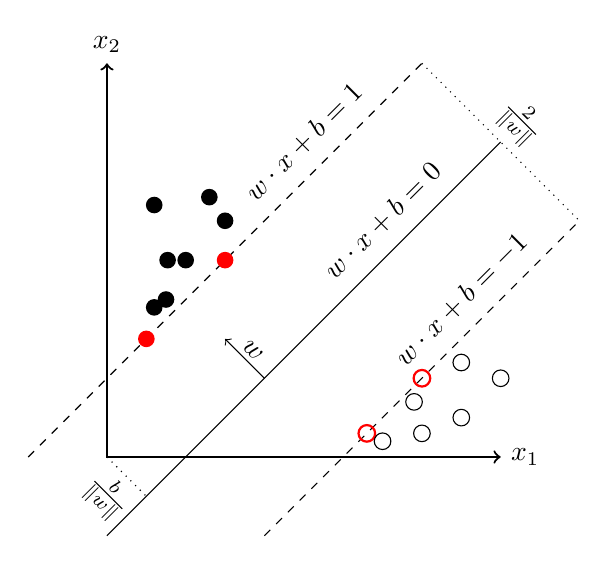
\begin{tikzpicture}
  % Draw axes
  \draw [<->,thick] (0,5) node (yaxis) [above] {$x_2$}
        |- (5,0) node (xaxis) [right] {$x_1$};
  % Draw line
  \draw (0,-1) -- (5,4); % y=x-1
  \draw[dashed] (-1,0) -- (4,5); % y=x+1
  \draw[dashed] (2,-1) -- (6,3); % y=x-3
  % Draw labels
  \draw (3.5,3) node[rotate=45] 
        {$w \cdot x + b = 0$};
  \draw (2.5,4) node[rotate=45] 
        {$w \cdot x + b = 1$};
  \draw (4.5,2) node[rotate=45] 
        {$w \cdot x + b = -1$};
  % Draw distance
  \draw[dotted] (4,5) -- (6,3);
  \draw (5.25,4.25) node[rotate=-45] {$\frac{2}{\Vert w \Vert}$};
  \draw[dotted] (0,0) -- (0.5,-0.5);
  \draw (0,-0.5) node[rotate=-45] {$\frac{b}{\Vert w \Vert}$};
  \draw[->] (2,1) -- (1.5,1.5);
  \draw (1.85,1.35) node[rotate=-45] {$w$};
  % Draw negative dots
  \fill[red] (0.5,1.5) circle (3pt);
  \fill[red]   (1.5,2.5)   circle (3pt);
  \fill[black] (1,2.5)     circle (3pt);
  \fill[black] (0.75,2)    circle (3pt);
  \fill[black] (0.6,1.9)   circle (3pt);
  \fill[black] (0.77, 2.5) circle (3pt);
  \fill[black] (1.5,3)     circle (3pt);
  \fill[black] (1.3,3.3)   circle (3pt);
  \fill[black] (0.6,3.2)   circle (3pt);
  % Draw positive dots
  \draw[red,thick] (4,1)     circle (3pt); 
  \draw[red,thick] (3.3,.3)  circle (3pt); 
  \draw[black]     (4.5,1.2) circle (3pt); 
  \draw[black]     (4.5,.5)  circle (3pt); 
  \draw[black]     (3.9,.7)  circle (3pt); 
  \draw[black]     (5,1)     circle (3pt); 
  \draw[black]     (3.5,.2)  circle (3pt); 
  \draw[black]     (4,.3)    circle (3pt); 
\end{tikzpicture}
\caption{Hyperplan optimal au sens de la marge \label{fig:svm} }
\end{figure}

Soit $\{ x_i , y_i \}_{i=1..N}$ l'échantillon d'apprentissage avec $x_i \in \mathbb{R}^n$ les vecteurs de données et $y_i \in \{-1,1\} $ sa classe. 
Si l'on suppose que le jeu de donné $ \{ x_i , y_i \}_{i=1..N} $ est linéairement séparable c'est-à-dire
\begin{equation*}
    \mathcal{U}_{\text{adm}} = \left\{ (w,b) | \forall i \; y_i ( w^\intercal x_i = b)\geq 1  \right\} \neq \emptyset
\end{equation*}
alors on peut définir l'hyperplan:
\begin{equation*}
    \left\{ x : f(x) := w^\intercal x + b = 0 \right\}
\end{equation*} 
Donc la règle de classification biclasse est $ \sgn [ f(x) ] $. On appelle alors hyperplan optimal un hyperplan qui maximise la marge, on à alors le problème d'optimisation convexe suivant:
\begin{equation*}
    \begin{aligned}
        & \text{minimiser}
        & & J_{w,b}(w) = \frac{1}{2} \| w \|^2 \\
        & \text{sous contraintes}
        & & y_i \left( w^\intercal x_i + b \right)\geq 1 , \; \forall i \leq N
    \end{aligned}
\end{equation*}
où la solution existe bien puisque $\mathcal{U}_{\text{adm}} \neq \emptyset$. On peut alors appliquer le théorème de \ac{kkt} pour caractériser les solutions $w^*$, $b^*$, $\lambda^*$ de ce problème et le Lagrangien correspondant est:

\begin{gather*}
    L (w,b,\lambda) = \frac{1}{2} \Vert w \Vert^2 + \sum_{j=1}^n \lambda_j ( 1 - y_j ( w^\intercal x_j + b )) \\
    \lambda_i\geq 0
\end{gather*}

La fonction duale du Lagrangien est:

\begin{equation*}
    \Theta (\lambda) = \min_{w,b} L (w,b,\lambda) = L (w^*,b^*,\lambda)
\end{equation*}

Pour trouver $w^*$ et $b^*$ on calcule le gradient et on obtient les conditions suivantes:

\begin{equation*}
    \nabla_w L (w,b,\lambda) = w - \sum_{j=1}^n \lambda_j y_j x_j = 0
\end{equation*}

Ce qui implique:

\begin{equation*}
    w^* = \sum_{j=1}^n \lambda_j y_j x_j
\end{equation*}

On a aussi :

\begin{equation*}
    \frac{ \partial L (w^*,b^*,\lambda)}{\partial b} =  - \sum_{j=1}^n \lambda_j y_j = 0
\end{equation*}

En réinjectant dans $L$ on a:

\begin{align*}
    L (w^*,b^*,\lambda) &= \sum_{j=1}^n \lambda_j - b \sum_{j=1}^n \lambda_j y_j - \frac{1}{2} \sum_{i=1}^n \sum_{j=1}^n \lambda_i \lambda_j y_i y_j x_i^\intercal x_j \\
    &= \sum_{j=1}^n \lambda_j - \frac{1}{2} \sum_{i=1}^n \sum_{j=1}^n \lambda_i \lambda_j y_i y_j x_i^\intercal x_j 
\end{align*}

Dans le cas non séparable, il n'existe pas de solution au problème puisque la solution est nécessairement un hyperplan de séparation.
\subsubsection{Cas non séparable}

On relâche alors la contrainte en autorisant certaines variables à se trouver dans la marge.
\begin{equation*}
    \begin{aligned}
        & \text{minimiser}
        & & J_{w,b,\xi} (w) = \frac{1}{2} \Vert w \Vert^2 + \overbrace{C \sum_{i=1}^n \xi_i}^{\textit{pénalisation}} \\
        & \text{sous contraintes}
        & & y_i \left( w^\intercal x_i + b \right)\geq 1 - \xi_i, \; \forall i \leq N  \\
        & & & \xi_i \geq 0 \\
    \end{aligned}
\end{equation*}

Le Lagrangien $L(w,b,\xi,\alpha,\lambda)$ est :

\begin{equation*}
    L(w,b,\xi,\alpha,\lambda) = \frac{1}{2} \Vert w \Vert^2 + C \sum_{i=1}^n \xi_i + \sum_{i=1}^n \alpha_i ( 1 - y_j ( w^\intercal x_i + b ) - \xi_i ) + \sum_{i=1}^n \lambda_i ( - \xi )
\end{equation*}

Sous contraintes $\alpha_i > 0$ et $\lambda_i > 0$. On dérive alors par rapport à $w$ et on obtient la condition:

\begin{equation*}
\begin{aligned}
    & & & \frac{\partial L}{\partial w} = w - \sum_{i=1}^n \alpha_i y_i x_i = 0 \\
    & \textit{i.e. }
    & & w = \sum_{i=1}^n \alpha_i y_i x_i
\end{aligned}
\end{equation*}

En dérivant par rapport à $b$ on obtient la condition:

\begin{equation*}
    \frac{\partial L}{\partial b} = \sum_i^n \alpha_i y_i = 0
\end{equation*}

Et par rapport à $\xi_i$ on a enfin:

\begin{equation*}
\begin{aligned}
    & & & \frac{\partial L}{\partial \xi_i} = C- \alpha_i - \lambda_i = 0 \\
    & \textit{i.e.}
    & & \alpha_i = C - \lambda_i
\end{aligned}
\end{equation*}

En réinjectant, on trouve alors:

\begin{equation*}
    \begin{aligned}
        & \text{maximiser}
        & & L_D = \sum_{i=1}^N \alpha_i - \frac{1}{2} \sum_{i=1}^N \sum_{j=1}^N \alpha_i \alpha_j y_i y_j \langle x_i , x_j \rangle \\
        & \text{sous contraintes}
        & & 0≤\alpha_i \leq C, \; \forall i \leq N  \\
        & & & \sum_{i=1}^N \alpha_i y_i = 0 \\
        & \text{La solution vérifie}
        & & w^* = \sum_{i=1}^N \alpha_i^* y_i x_i \\
        & & & f(x) = \sum_{i=1}^N \alpha_i^* y_i \langle x_i,x \rangle + b \\
    \end{aligned}
\end{equation*}

On peut résoudre ce problème en réappliquant le théorème de \ac{kkt} sur ce problème plus simple ne comportant plus qu'une variable au lieu de $3$ ou par tout autre algorithme de résolution numérique comme Sequential minimal optimization tel que dans \citet{Platt}.

\subsection{Non-linéarité et noyaux}
\subsubsection{Motivation}

\begin{figure}[htbp]
\centering
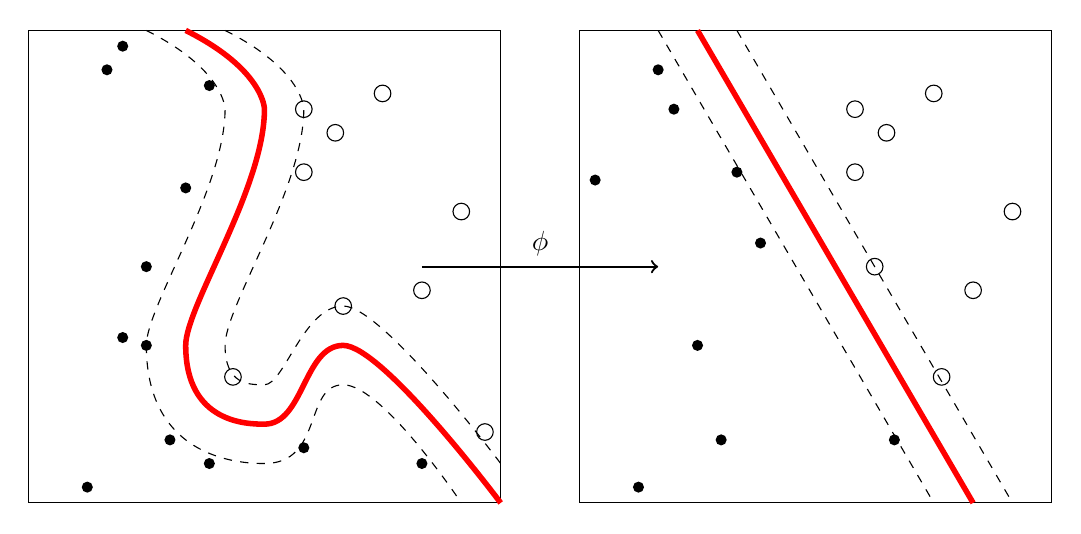
\begin{tikzpicture}[x=1cm,y=1cm]

%draw[color=gray] (0,0) grid (6,6);
\draw (0,0) rectangle (6,6);
% Draw line
\draw[color=red,line width=2pt]
  (2,6) .. controls (3,5.5) and (3,5) .. 
  (3,5) .. controls (3,4) and (2,2.5) .. 
  (2,2) .. controls (2,1) and (2.8,1) .. 
  (3,1) .. controls (3.5,1) and (3.5,2) .. 
  (4,2) .. controls (4.5,2) and (6,0) .. 
  (6,0);
% Draw left dashed line
\draw[dashed] 
  (1.5,6) .. controls (2.5,5.5) and (2.5,5) .. 
  (2.5,5) .. controls (2.5,4) and (1.5,2.5) .. 
  (1.5,2) .. controls (1.5,.5) and (2.8,.5) .. 
  (3,.5) .. controls (3.75,.5) and (3.5,1.5) .. 
  (4,1.5) .. controls (4.5,1.5) and (5.5,0) .. 
  (5.5,0);
% Draw right dashed line
\draw[dashed] 
  (2.5,6) .. controls (3.5,5.5) and (3.5,5) .. 
  (3.5,5) .. controls (3.5,4) and (2.5,2.5) .. 
  (2.5,2) .. controls (2.5,1.5) and (2.8,1.5) .. 
  (3,1.5) .. controls (3.25,1.5) and (3.5,2.5) .. 
  (4,2.5) .. controls (4.5,2.5) and (6,0.5) .. 
  (6,0.5);
%draw[color=gray] (2,6) -- (3,5) -- (2,2) -- (3,1) -- (4,2) -- (6,0);
%draw[color=gray] (1.5,6) -- (2.5,5) -- (1.5,2) -- (3,.5)-- (4,1.5)-- (5.5,0);
%draw[color=gray] (2.5,6) -- (3.5,5) -- (2.5,2) -- (3,1.5)-- (4,2.5)-- (6,0.5);

%draw[color=gray] (7,0) grid (13,6);
\draw (7,0) rectangle (13,6);
% Draw line
\draw[color=red,line width=2pt] (8.5,6) -- (12,0);
% Draw dashed line
\draw[dashed]  (8,6) -- (11.5,0);
\draw[dashed]  (9,6) -- (12.5,0);

\draw[->,thick] (5,3) -- (8,3) node [above,pos=.5] {$\phi$};

\def \positive{{%
{2.3,5.3},
{3.5,.7},
{1.5,2},
{1.2,2.1},
{1.8,.8},
{1,5.5},
{1.2,5.8},
{.75,.2},
{2,4},
{5, 0.5},
{1.5,3},
{2.3,.5},
%
{9.3,3.3},
{11,.8},
{8.5,2},
{7.2,4.1},
{8.8,.8},
{8,5.5},
{8.2,5},
{7.75,.2},
{9,4.2},
{12, 0.5},
{8.5,3},
{9.3,.5},
}}

% Draw positive dots
\foreach \i in {0,...,20} {
  \pgfmathparse{\positive[\i][0]}\let \x \pgfmathresult;
  \pgfmathparse{\positive[\i][1]}\let \y \pgfmathresult;
  \fill[black] (\x,\y) circle (2pt);
}

\def \negative{{%
{4,2.5},
{3.5,5},
{2.6,1.6},
{4.5,5.2},
{5.5,3.7},
{3.9,4.7},
{5,2.7},
{3.5,4.2},
{5.8,.9},
%
{10.75,3},
{10.5,5},
{11.6,1.6},
{11.5,5.2},
{12.5,3.7},
{10.9,4.7},
{12,2.7},
{10.5,4.2},
{12.8,.9},
}}

% Draw negative dots
\foreach \i in {0,...,16} {
  \pgfmathparse{\negative[\i][0]}\let \x \pgfmathresult;
  \pgfmathparse{\negative[\i][1]}\let \y \pgfmathresult;
  \draw[black] (\x,\y) circle (3pt);
}
\end{tikzpicture}
\caption{Transformation d'un problème non linéaire en problème linéaire dans un espace de dimension supérieure}
\end{figure}

Il est également possible de séparer les classes non linéairement en se plaçant sur un espace de dimension supérieure. En effet on a le théorème suivant dû à \citet{Cover1965}.

\begin{theoreme}[Cover]
La probabilité que les classes soient linéairement séparables augmente quand les vecteurs sont non linéairement appliqués à un espace de dimension supérieure.
\end{theoreme}

\begin{hproof}
Pour $N$ individus distincts dans un espace $l$-dimensionnel, le nombre de groupements linéairement séparables est:
\begin{equation*}
    O(N,l) = 2 \sum_{i=0}^l \binom{N-1}{i}
\end{equation*}
alors que le nombre total de groupements est $2^N$. Alors la probabilité que l'échantillon soit linéairement séparable est le rapport
\begin{equation*}
    P^l_N = \frac{O(N,l)}{2^N}
\end{equation*}
\end{hproof}

\todo{Faire jolie preuve}

En effet une surface de séparation admissible dans cet espace de dimension supérieure reste une surface de séparation dans notre espace de départ lorsque transportée par une fonction injective.

\subsubsection{SVMs non linéaires}
Il est alors légitime d'appliquer notre séparation SVM dans un espace de dimension supérieur. Notre problème devient alors:

\begin{equation*}
    \begin{aligned}
        & \text{maximiser}
        & & L_D = \sum_{i=1}^N \alpha_i - \frac{1}{2} \sum_{i=1}^N \sum_{j=1}^N \alpha_i \alpha_j y_i y_j \langle \phi(x_i) , \phi(x_j) \rangle \\
        & \text{sous contraintes}
        & & 0≤\alpha_i≤\gamma, \; \forall i \leq N  \\
        & & & \sum_{i=1}^N \alpha_i y_i = 0 \\
        & \text{solution}
        & & w^* = \sum_{i=1}^N \alpha_i^* y_i \phi(x_i) \\
        & & & f(x) = \sum_{i=1}^N \alpha_i^* y_i \langle \phi(x_i),\phi(x) \rangle + b \\
    \end{aligned}
\end{equation*}

Néanmoins cette technique comporte de nombreux inconvénients; en se plaçant en haute dimension le calcul de $\phi$ devient de plus en plus complexe. Qui plus est, cela suppose que l'on soit capable de trouver $\phi$ manuellement, c'est notamment le cas lorsque $\langle \phi(x_i) , \phi(x_j) \rangle$ peut s'écrire $K(x_i,x_j)$, c'est ce qu'on appellera un noyau. 

Donnons néanmoins un exemple simple pour lequel il est possible de trouver explicitement $\phi$. Le cas de deux disques de points concentriques séparables par un ellipsoïde. On choisit comme noyau:
\begin{equation*}
    K(x,y) = \left( x^\intercal y \right)^2
\end{equation*}

que l'on peut associer à la fonction de transport $\phi$ suivante: 

\begin{equation*}
    \phi(x) = \left( x_1^2, x_2^2, \sqrt{2} x_1 x_2 \right)
\end{equation*}

\subsubsection{Kernel Trick}
On peut remarquer que le programme d'optimisation linéaire ne fait intervenir que le produit scalaire des $ \phi(x_i) $. On va donc montrer l'existence de fonctions $\phi$ telles que:
\begin{equation*}
    K(x_i,x_j) = \langle \phi(x_i) , \phi(x_j ) \rangle
\end{equation*}
où $K$ est une fonction donnée que l'on appelle noyau. On peut donc se contenter dans ce cas de faire tous nos calculs dans l'espace d'origine à l'aide de $K$. Une condition suffisante pour l'existence de $\phi$ est que $K$ soit symétrique défini positif.

\begin{definition}[Définie Positivité]
Une fonction symétrique $K : \mathcal{X} \times \mathcal{X} \rightarrow \mathbb{R} $ est définie positive si pour toute suite finie de points $x_1,\dots,x_n$ de $\mathcal{X}$ et tout choix des réels $c_1,\dots, c_n$ on a:
\begin{equation*}
    \sum_{i=1}^n \sum_{j=1}^n c_i K(x_i,x_j) c_j > 0
\end{equation*}
\end{definition}

\subsection{Espace de Hilbert à noyau reproduisant}

Un \ac{rkhs} \citep{Aronszajn1950}, est un espace de Hilbert $\mathcal{H}$ dans lequel toutes les fonctions d'évaluation de Dirac de $\mathcal{H}$ sont bornées et continues pour la norme $L^2$. Par le théorème de Riesz, on a l'existence d'un unique $k_x \in \mathcal{H}$ tel que $\delta_x f = f(x) = \langle f, k_x \rangle_{\mathcal{H}}$ pour tout $f \in \mathcal{H}$. On définit alors le \textit{Noyau Reproduisant} $K$ de $\mathcal{H}$ par: $ K(x,x') = \langle k_x , k_{x'} \rangle_{\mathcal{H}} $. La propriété importante des \ac{rkhs} est que $ \langle f , K(x,\cdot) \rangle_{\mathcal{H}} = f(x)$. Qui plus est, $k_x$ est défini comme étant la fonction $ y \rightarrow K(x,y) $ et donc $ \langle K(x,\cdot), K(y,\cdot) \rangle_{\mathcal{H}} = K(x,y) $

\subsubsection{Créer un \ac{rkhs} à partir d'un noyau}

On a vu que les noyaux reproduisants étaient définis positifs puisqu'ils étaient des produits scalaires, nous allons montrer qu'en réalité toute fonction définie positive est le noyau reproduisant d'un certain espace $\mathcal{H}_K$ unique à un isomorphisme près.

Considérons $\mathcal{H}_K = \overline{\vect S} $ ou $ S = \{ k_{x_i} = K(x_i,\cdot) : x_i \in X \} $. On définit alors un produit scalaire sur $\mathcal{H}_K$ de la manière suivante: soient $f$,$g$ tels que:
\begin{align*}
    &f(x) = \sum_{i=1}^\infty \alpha_i K(x,x_i) \in \mathcal{H}_K \\
    &g(x) = \sum_{i=1}^{\infty} \beta_i K(x,x'_i) \in \mathcal{H}_K
\end{align*}
alors:
\begin{equation*}
    \langle f , g \rangle_{\mathcal{H}_K} :=  \sum_{i=1}^\infty \sum_{j=1}^{\infty} \alpha_i \beta_j K(x_i,x'_j)
\end{equation*}

Il est aisé de voir que $\langle \cdot , \cdot \rangle_{\mathcal{H}_K}$ définit un produit scalaire. Donc on a:

\begin{align*}
    \langle f , K(\cdot,x) \rangle_{\mathcal{H}_K} &= \sum_{i=1}^n \sum_{j=1}^{n'} \alpha_i K(x,x_i) \\
    &=  f(x)
\end{align*}
Et en particulier
\begin{equation*}
    \langle K(\cdot,x) , K(\cdot,y) \rangle_{\mathcal{H}_K} =  K(x,y)
\end{equation*}

Donc dans cette construction on a: $\phi (x) = K(\cdot,x)$

\subsubsection{Construction de Mercer}

On rappelle d'abord le théorème dû à \citet{Mercer}

\begin{theoreme}[Theorème de Mercer]
Supposons que $K$ est un noyau continu symétrique défini positif sur $X$. Si la fonction $k$ ou $k(x) = K(x,x)$ est $L^1_\mu (X)$ alors il existe une base orthonormée $(e_i)_{i\in \mathbb{N}}$ de $L^2_{\mu} (X)$ de fonctions propres de $T_K$

\begin{equation*}
    [T_K \varphi](x) =\int_\mu  K(x,s) \varphi(s)\, \diff \mu (s)
\end{equation*}
 
telles que la suite de valeurs propres $(\lambda_i)_{i \in \mathbb{N}}$ soit positive. Les fonctions propres associées à des valeurs propres non nulles sont continues sur $X$ et $K$ possède la représentation suivante:

\begin{equation*}
    K(s,t) = \sum_{j=1}^\infty \lambda_j \, e_j(s) \, e_j(t)
\end{equation*}
\end{theoreme}

On peut alors utiliser cette représentation bien particulière pour construire un \ac{rkhs}. Considérons un noyau $K(x,x')$ semi-défini positif. D'après le théorème de Mercer, il existe une famille orthonormée par rapport à une mesure $\mu$ quelconque de fonctions propres $\psi_i$ telle que
\begin{equation*}
    K(x,x') = \sum_{i=1}^\infty \lambda_i \psi_i (x) \psi_i (x')
\end{equation*}
Considérons maintenant l'espace de Hilbert: 
\begin{equation*}
    \mathcal{H}_K = \{f | f(x) = \sum_{i=1}^\infty f_i \psi_i (x) , \sum_{i=1}^\infty f_i^2 / \lambda_i < \infty \}
\end{equation*}
muni du produit scalaire suivant:
\begin{equation*}
    \langle f,g \rangle_{\mathcal{H}} = \sum_{i=1}^\infty \frac{f_i g_i}{\lambda_i}
\end{equation*}
Le caractère reproduisant en découle aisément:
\begin{align*}
    \langle f(\cdot) , K(\cdot,x) \rangle &= \sum_{i=1}^\infty \frac{f_i \lambda_i \psi_i (x)}{\lambda_i} \\
    &= f(x)
\end{align*}
De la même façon:
\begin{align*}
    \langle K(\cdot,x) , K(\cdot,x') \rangle &= \sum_{i=1}^\infty \frac{\lambda_i \psi_i (x) \lambda_i \psi_i (x')}{\lambda_i} \\
    &= K(x,x')
\end{align*}

De plus $K(x,\cdot) \in \mathcal{H}$ puisque $ \| K(x,\cdot) \| = K(x,x) < \infty $. Et on pose enfin
\begin{equation*}
    \phi(x) = \left( \sqrt{\lambda_1} \psi_1 (x) , \dots , \sqrt{\lambda_n} \psi_n (x) \right)
\end{equation*}

\subsection{Théorème de représentation}

On vient donc de voir l'utilité des \ac{rkhs} dans le cas bien précis des SVM. Mais le théorème de représentation prouvé par \citet{Scholkopf2001} permet de généraliser cette méthode à d'autres problèmes d'optimisation similaires.

\begin{theoreme}[Théorème de représentation]
Soit $\mathcal{X}$ un ensemble non vide et $K$ un noyau réel symétrique non défini positif sur $\mathcal{X} \times \mathcal{X}$ avec un \ac{rkhs} correspondant $\mathcal{H}_K$.
Étant donné un échantillon d'apprentissage $(x_i, y_i)_i \in \mathcal{X} \times \mathbb{R}$, une fonction réelle strictement croissante $g \colon [0, \infty) \to \mathbb{R}$, et une fonction de risque empirique quelconque $E \colon (\mathcal{X} \times \mathbb{R}^2)^n \to \mathbb{R} \cup \lbrace \infty \rbrace$, alors pour n'importe quel $f^{*} \in H_k$ satisfaisant
\begin{equation*}
    f^{*} = \argmin_{f \in H_k} \left\{ E\left( (x_1, y_1, f(x_1)), ..., (x_n, y_n, f(x_n)) \right) + g\left( \Vert f \Vert \right) \right\}
\end{equation*}
$f^{*}$ admet une représentation de la forme:
\begin{equation*}
    f^{*}(\cdot) = \sum_{i = 1}^n \alpha_i K(\cdot, x_i)
\end{equation*}
où $\alpha_i \in \mathbb{R}$ pour tout $1 \le i \le n$.
\end{theoreme}

On peut donc en réalité étendre grâce aux \ac{rkhs} les techniques étudiées précédemment à un bien plus vaste champ de problèmes d'optimisation et donc de techniques de classification. Les très bons résultats des \ac{svm}s en font une technique de choix pour un très grand nombre de problèmes, mais ceux-ci ne sont pas exempts de problèmes, en effet les performances dépendent grandement du noyau choisi et il est donc nécessaire d'adapter la structure du classifieur au jeu de données et au problème étudié. De plus les \ac{svm}s restent une technique "boîte noire" qui ne fournit aucune information explicative sur le modèle sous-jacent et le contributions des variables. Enfin comme beaucoup de modèles, elles sont très sensibles à l'overfitting si un noyau trop discriminant est choisi ainsi qu'au déséquilibre des données.

\section{Les réseaux de neurones}

Les réseaux de neurones, ainsi nommés, car apparus simultanément et indépendamment dans la communauté neuro-scientifique et statistique, peuvent être vus comme une généralisation des méthodes linéaires. En effet, là où celles-ci considèrent des combinaisons linéaires de fonctions des entrées comme première généralisation, les réseaux de neurones répètent ce principe $n$ fois en considérant chaque nouvelle sortie comme une nouvelle entrée.

\subsection{Principe}

Un réseau de neurones est organisé en un certain nombre de \emph{couches} de neurones, ces derniers étant définis par $\left( \omega_{ik}^{l+1} \right)_i$ le vecteur des poids de sorties du $k^\text{ème}$ neurone de la couche $l$ et $b_ik^l$ son biais. Nous ne considérons ici que les réseaux entièrement connectés c'est-à-dire tels que chaque neurone de la couche $l$ pointe vers tous les neurones de la couche $l+1$. Ainsi chaque neurone reçoit les sorties de tous les neurones précédents et fournit en sortie à tous les neurones suivant la valeur $a_k^l$:
\begin{equation*}
    a_k^l = \sigma \left( \sum_j \omega^l_{kj} a^{l-1}_j + b^l_k \right)
\end{equation*}
Pour simplifier les notations, on notera par $\omega^l$ la matrice des poids de la couche $l$, $b^l$ le vecteur des biais et $a^l$ le vecteur des sorties. Ici $\sigma$ est une fonction à choisir en fonction du problème appelée fonction d'activation.

\def\layersep{2.5cm}
\begin{figure}[htbp]
\centering
\begin{tikzpicture}[shorten >=1pt,->,draw=black, node distance=\layersep]
    \tikzstyle{every pin edge}=[<-,shorten <=1pt]
    \tikzstyle{neuron}=[circle,draw,thick,minimum size=17pt,inner sep=0pt]
    \tikzstyle{input neuron}=[neuron];
    \tikzstyle{output neuron}=[neuron];
    \tikzstyle{hidden neuron}=[neuron];
    \tikzstyle{annot} = [text width=4em, text centered]

    % Draw the input layer nodes
    \foreach \name / \y in {1,...,4}
    % This is the same as writing \foreach \name / \y in {1/1,2/2,3/3,4/4}
        \node[input neuron, pin=left:$x_\y$] (I-\name) at (0,-\y) {};

    % Draw the hidden layer nodes
    \foreach \name / \y in {1,...,5}
        \path[yshift=0.5cm]
            node[hidden neuron] (H-\name) at (\layersep,-\y cm) {};

    % Draw the output layer node
    \node[output neuron,pin={[pin edge={->}]right:$y$}, right of=H-3] (O) {};

    % Connect every node in the input layer with every node in the
    % hidden layer.
    \foreach \source in {1,...,4}
        \foreach \dest in {1,...,5}
            \path (I-\source) edge (H-\dest);

    % Connect every node in the hidden layer with the output layer
    \foreach \source in {1,...,5}
        \path (H-\source) edge (O);

    % Annotate the layers
    \node[annot,above of=H-1, node distance=1cm] (hl) {Couche cachée};
    \node[annot,left of=hl] {Couche d'entrée};
    \node[annot,right of=hl] {Couche de sortie};
\end{tikzpicture}
\caption{Réseau de neurones artificiel $4\times 5 \times 1$ } \label{fig:rnn}
\end{figure}

Ainsi la sortie $\hat{y} = a^L$ est définie de manière récursive:
\begin{align*}
    a^1 &= x \\
    a^l &= \sigma(\omega^l a^{l-1} + b^l )
\end{align*}

\todo{Comment est donnée la sortie...?????}

Comme dans les autres algorithmes d'apprentissage, on va alors chercher à apprendre $\omega^l$ et $b^l$ afin de minimiser une certaine fonction de perte $J (y,\hat{y})$, la plupart du temps la perte $L^2$. En effet cette tache est légitime puisqu'il est possible de montrer qu'un tel réseau de neurones est capable d'approcher toute fonction continue sur un compact sous certaines hypothèses \citep{Hornik1991}.

\begin{theoreme}[\cite{Cybenko}]
    Soit $\sigma$ une fonction sigmoïde continue. Soit $I_m = [0,1]^m$ l'hypercube de dimension $m$ et $\mathcal{C} (I_m)$ l'espace des fonctions continues sur $I_m$. Alors pour tout $f \in \mathcal{C} (I_m)$, $\varepsilon > 0$ il existe un entier $N$ et $v_i, b_i \in \mathbb{R}$, $\omega_i \in \mathbb{R}^m$ tel que:
    \begin{equation*}
    \begin{aligned}
        & & & \vert \varphi(x) - f(x)  \vert < \varepsilon , \forall x \in I_m \\
        & \text{avec}
        & & \varphi(x) = \sum_{i=1}^N v_i \sigma ( \omega_i^\intercal + b_i )
    \end{aligned}
    \end{equation*}
\end{theoreme}

\begin{proof}
    La preuve~\ref{cybenko} de \citet{Cybenko} procède en deux étapes en montrant tout d'abord que les fonctions discriminantes pour les mesures sont denses dans $\mathcal{C} (I_m)$ puis que les fonctions sigmoïdes sont discriminantes pour les mesures.
\end{proof}

Le problème d'apprentissage des réseaux de neurones n'est alors qu'un problème d'optimisation en les $\omega_i, b_i$ que l'on peut résoudre par descente de gradient. Néanmoins le nombre colossal de coefficients et biais à optimiser résulte en autant de dérivées partielles à calculer, le problème ne peut donc pas être résolu de manière naïve en un temps raisonnable. Nous allons donc voir en quoi la forme particulière du réseau de neurones et donc de la fonction de sortie permet de mettre en place un algorithme d'optimisation rapide.

\todo{REVOIR TOUTES LES NOTATIONS + REFAIRE CALCULS}

\subsection{Rétropropagation}

On se place ici dans le cas où la fonction de perte pour l'échantillon d'apprentissage entier s'exprime comme la moyenne des pertes pour chaque individu et où la perte pour un seul individu peut s'écrire comme fonction des sorties du réseau. On suppose de plus que la perte est différentiable. C'est par exemple le cas pour la perte quadratique que nous utiliserons à partir d'ici. Nous n'exposerons qu'une version simplifiée des réseaux de neurones \emph{feed-forward} sans aborder les subtilités telles que le \emph{dropout} et la régularisation. Pour de plus amples informations il est possible de consulter \citep{Rojas1996,Nielsen2015,Bengio2015}.

On cherche à optimiser les poids et biais afin de minimiser la perte, on procède alors par descente de gradient. Il faut alors pour cela calculer le gradient de la perte par rapport aux poids et biais. Le calcul du gradient pourrait se faire par différence finie, ce qui serait non seulement très coûteux, car nécessitant $O (n)$ opérations où $n$ est le nombre de paramètres a optimiser, mais également imprécis. Il est également possible d'effectuer une différentiation symbolique soit à la main, soit par ordinateur. Dans notre cas il est finalement possible d'exploiter la structure très particulière du problème.

Si l'on appelle $\theta$ l'ensemble des paramètres, la procédure est alors:
\begin{equation*}
    \Delta \theta = -\gamma \nabla_{\theta} C
\end{equation*}
ou $\gamma$ est la vitesse d'apprentissage.

Or un réseau de neurones représente un graphe de composition de fonctions, nous allons donc utiliser les propriétés de la différentielle d'une composée de fonctions pour faciliter les calculs.

Notons $z^l_j = \sum_k \omega^l_{jk} a^{l-1}_k + b^l_j$ et l'\emph{erreur} locale $\delta^l_j \equiv \frac{\partial C}{\partial z^l_j}$.

En utilisant la formule de la dérivée d'une fonction composée on trouve les équations de la rétropropagation qui permettent de calculer l'\emph{erreur} et donc les dérivées partielles à chaque nœud en remontant le graphe de manière rétrograde.

\begin{theoreme}[Équations de la rétropropagation]
    \begin{gather}
        \delta^L = \nabla_a C \odot \sigma' (z^L ) \\
        \delta^l = \left( \left( \omega^{l+1} \right)^\intercal \delta^{l+1} \right) \odot \sigma' ( z^l ) \\
        \frac{\partial C}{\partial b^l_j} = \delta^l_j \\
        \frac{\partial C}{\partial \omega^l_{jk}} = a^{l-1}_k \delta^l_j
    \end{gather}
    Ou $\odot$ est le produit d'Hadamard ou de Schur, c'est à dire le produit composante par composante.
\end{theoreme}

\todo{Faire la preuve. Assez simple. Bien vérifier les indices}

En utilisant les équations de rétropropagation il est alors possible de calculer le gradient par rapport à tous les paramètres en un seul parcours du graphe et de façon indépendante au sein de chaque couche, donc entièrement en parallèle au sein de chaque couche. Ainsi le problème d'optimisation d'origine qui paraissait intraitable en un temps raisonnable peut maintenant être résolu en un temps tolérable. De plus, la capacité à hautement paralléliser l'algorithme permet, contrairement à d'autres problèmes en apparence plus simple, de diminuer le temps de calcul de façon arbitraire en rajoutant des unités de calcul, la seule contrainte étant alors les moyens financiers dont on dispose.

\subsection{Différentiation automatique}

Nous avons vu une méthode pour calculer les dérivées d'une fonction en apparence très complexe en un temps de calcul limité et sans commettre aucune erreur due aux approximations numériques. Nous allons maintenant voir que cette technique n'est pas limitée aux réseaux de neurones et peut s'appliquer sous deux formes à différents problèmes de calcul de gradient ou dérivées supérieures tels que présents en finance, voir par exemple \citet{Homescu2011}, \citet{Giles2005} ou \citet{Xu2014}.

En effet, de la même façon que dans le cas des réseaux de neurones il est toujours possible d'exprimer une fonction complexe comme un graphe de composition de fonctions de base. Nous allons donc utiliser les propriétés de la différentiation de composées de fonctions.

\begin{figure}[htbp]
\begin{tikzpicture}[->,>=stealth',shorten >=1pt,auto,node distance=1.5cm,
  thick,main node/.style={circle,draw}, function node/.style={rectangle,draw}]

  \node[main node] (1) {$x$};
  \node[function node] (2) [right of=1] {$\exp ( \cdot )$};
  \node[main node] (3) [right of=2] {$u_1$};
  \node[function node] (4) [above of=3] {$(\cdot)^2$};
  \node[main node] (5) [right of=4] {$u_2$};
  \node[function node] (6) [right of=3] {$+$};
  \node[main node] (7) [right of=6] {$u_3$};
  \node[function node] (8) [above right of=7] {$\sin (\cdot)$};
  \node[function node] (9) [below right of=7] {$\exp ( \cdot )$};
  \node[main node] (10) [right of=8] {$u_4$};
  \node[main node] (11) [right of=9] {$u_5$};
  \node[function node] (12) [below right of=10] {$+$};
  \node[main node] (13) [right of=12] {$y$};

  \path
    (1) edge (2)
    (2) edge (3)
    (3) edge (4)
    (4) edge (5)
    (5) edge (6)
    (3) edge (6)
    (6) edge (7)
    (7) edge (8)
    (7) edge (9)
    (8) edge (10)
    (9) edge (11)
    (10) edge (12)
    (11) edge (12)
    (12) edge (13);
\end{tikzpicture}
\caption{Graphe de $f(x) = \exp ( \exp(x) + (\exp(x))^2 ) + \sin ( \exp(x) + (\exp(x))^2 )$}\label{fig:graphe.fonction}
\end{figure}

Prenons par exemple le cas de~\ref{fig:graphe.fonction}. Nous pouvons traverser le graphe de gauche à droite, ou de droite à gauche.

\subsubsection{Backward}

On peut alors réécrire le graphe sous forme équationelle:
\begin{align*}
    y &= f_6 ( u_5, u_4 ) &\diff y &= \frac{\partial f_6}{\partial u_5} \diff u_5 + \frac{\partial f_6}{\partial u_4} \diff u_4 \\
    u_5 &= f_5 ( u_3 ) &\diff u_5 &= \frac{\partial f_5}{\partial u_3} \diff u_3 \\
    u_4 &= f_4 ( u_3 ) &\diff u_4 &= \frac{\partial f_4}{\partial u_3} \diff u_3 \\
    u_3 &= f_3 ( u_2, u_1 ) &\diff u_3 &= \frac{\partial f_3}{\partial u_2} \diff u_2 + \frac{\partial f_3}{\partial u_1} \diff u_1 \\
    u_2 &= f_2 ( u_1 ) &\diff u_2 &= \frac{\partial f_2}{\partial u_1} \diff u_1 \\
    u_1 &= f_1 ( x ) &\diff u_1 &= \frac{\partial f_1}{\partial u_1} \diff u_1
\end{align*}

Il est ainsi aisé de voir que l'on peut obtenir $\frac{\partial y}{\partial x}$ en remontant le graphe par la droite, ce sens de calcul des dérivées dans le sens opposé du calcul de la fonction donne alors la différentiation automatique \emph{backward}. L'algorithme s'applique à toutes les fonctions $f : \mathbb{R}^n \rightarrow \mathbb{R}^m $, la différentiation automatique \emph{backward} est capable de calculer le gradient de chaque application partielle en une seule passe, mais nécessite $m$ passes pour le gradient complet. L'algorithme est donc intéressant dans le cas où $n \gg m$.

\todo{possible de rajouter une représentation graphique de l'algorithme ??}

\subsubsection{Forward}

Nous venons de voir une méthode permettant de calculer les dérivées en parcourant le graphe dans le sens inverse de l'évaluation de la fonction, mais il est également possible de mettre à jour l'état actuel de la dérivée en même temps que l'on traverse le graphe pour calculer la fonction. Puisqu'ici les deux calculs ont lieu dans le même sens on parle de différentiation automatique \emph{forward}.
Pour cela on augmente les nombres réels en les munissant de $\varepsilon$ avec $\varepsilon^2 = 0$. $\mathbf{x}$ appartient à la nouvelle algèbre obtenue appelée algèbre duale si $\mathbf{x} = x + x' \varepsilon$, $x,x' \in \mathbb{R}$.

Il est aisé de voir que si $P$ est un polynôme réel alors:
\begin{equation*}
    P(x+x' \varepsilon) = P(x) + P'(x) x' \varepsilon
\end{equation*}
Ainsi en étendant les fonctions analytiques à cette nouvelle algèbre nous avons un moyen d'obtenir à la fois la valeur de la fonction et sa dérivée en ce point en l'évaluant dans l'algèbre augmentée. Ainsi si $\bar{f}_i$ est l'extension de $f_i$ à notre nouvelle algèbre alors calculer $f = f_n \circ f_{n-1} \circ \dotsc \circ f_1$ ainsi que sa dérivée en $x$ revient à calculer $\bar{f}_n \circ \bar{f}_{n-1} \circ \dotsc \circ \bar{f}_1 ( x + 1 \varepsilon )$

La différentiation automatique \emph{forward} est très facile à implémenter et, comme la version \emph{backward}, s'étend au cas multidimensionnel. Néanmoins l'algorithme part ici d'une valeur d'entrée $x_i$ pour obtenir toutes les dérivées des fonctions partielles par rapport à celle-ci, il faut donc $n$ passes pour calculer le gradient entier et l'algorithme est intéressant dans le cas où $n \ll m$.
